\documentclass[11pt]{scrartcl}
\usepackage{graphicx}
\graphicspath{{./}}
\usepackage[sexy]{evan}
\usepackage[normalem]{ulem}
\usepackage{hyperref}
\usepackage{mathtools}
\hypersetup{
    colorlinks=true,
    linkcolor=blue,
    filecolor=magenta,      
    urlcolor=cyan,
    pdfpagemode=FullScreen,
    }

\renewcommand{\dangle}{\measuredangle}

\renewcommand{\baselinestretch}{1.5}

\addtolength{\oddsidemargin}{-0.4in}
\addtolength{\evensidemargin}{-0.4in}
\addtolength{\textwidth}{0.8in}
% \addtolength{\topmargin}{-0.2in}
% \addtolength{\textheight}{1in} 


\setlength{\parindent}{0pt}

\usepackage{pgfplots}
\pgfplotsset{compat=1.15}
\usepackage{mathrsfs}
\usetikzlibrary{arrows}

\title{Game Theory}
\author{Pelatihan OSP}
\date{April 2023}

\begin{document}

\maketitle
\begin{soaljawab}
    Akira dan Benjiro mempunyai tak hingga banyaknya koin bundar yang identik. Akira dan Benjiro bergantian menaruh koin tersebut di meja persegi yang ukurannya terbatas (finit) sehingga tidak ada dua koin yang saling bertumpuk dan setiap koin tepat di atas meja (jadi tidak ada yang koin yang menggantung di pinggiran meja sehingga bisa jatuh). Orang yang tidak bisa menempatkan koin di meja saat gilirannya dinyatakan kalah. Asumsikan setidaknya satu koin dapat ditaruh di meja. Jika Akira main duluan, buktikan bahwa Akira punya strategi menang.\\[-10pt]
    
    \begin{solusi}
    Akan ditunjukkan bahwa Akira punya strategi menang. Pertama, Akira menaruh koin tepat di tengah meja. Lalu, untuk selanjutnya setiap Benjiro menaruh koin di titik $K$ (selain di tengah meja), maka Akira akan mengikuti menaruh koin di titik $K'$ dimana $K'$ adalah pencerminan dari titik $K$ terhadap titik tengah meja. Dari kesimetrisan tersebut, dapat dipastikan bahwa Akira selalu dapat menaruh koinnya setelah Benjiro menaruh koin. Karena mejanya mempunyai ukuran terbatas, maka suatu saat setelah beberapa giliran, akan ada orang yang kalah karena tidak dapat menaruh koinnya. Karena Akira pasti dapat selalu menaruh koinnya, maka pasti Benjiro kalah dan Akira menang. Terbukti. \qed
    \end{solusi}
\end{soaljawab}

\begin{soaljawab}
Xeratha dan Haxuv sedang memainkan Cram, dimana giliran pertama dimainkan Xeratha dan mereka bergantian menempatkan domino (ubin berukuran $1 \times 2$ atau $2 \times 1$) pada grid persegi panjang $m \times n$ dan $mn$ bernilai genap. Xeratha maupun Haxuv harus menempatkan ubin domino secara vertikal atau horizontal, dengan ubin domino tersebut tidak boleh tumpang tindih atau keluar dari papan. Pemain yang tidak bisa melakukan langkah untuk pertama kalinya dinyatakan kalah dan pemain yang dapat melakukan langkah terakhir dinyatakan sebagai pemenang. Jika diberikan $m$ dan $n$, tentukan siapa yang memiliki strategi kemenangan, dan jelaskan strateginya.
    \begin{solusi}
        Perhatikan bahwa haruslah setidaknya salah satu dari $m$ dan $n$ bernilai genap. Haxuv memiliki strategi menang saat $m$ dan $n$ keduanya genap. Sedangkan Xeratha memiliki strategi menang saat tepat salah satu dari $m$ dan $n$ genap.
        \begin{itemize}
            \item Kasus $m$ dan $n$ keduanya genap. Saat Xeratha meletakkan domino pada gilirannya di posisi $k$, Haxuv dapat meletakkan domino di posisi $k'$ yang posisinya merupakan pencerminan $k$ terhadap pusat dari persegi panjang. Dari sini, untuk setiap gerakan yang dilakukan Xeratha, Haxuv dapat melakukan gerakan juga. Oleh karena itu Haxuv dijamin dapat terus melakukan gilirannya sampai habis. Dapat disimpulkan Haxuv mempunyai strategi menang untuk kasus ini.
            \item Kasus tepat salah satu dari $m$ dan $n$ genap. Tanpa mengurangi keumuman, misalkan $m=2t+1$ ganjil untuk suatu $t$ bulat nonnegatif dan $n=2r$ genap untuk suatu Rayyan asli. Xeratha pada giliran pertamanya dapat meletakkan domino tepat di tengah persegi panjang, atau di baris ke $t+1$ dan di kolom Rayyan sampai $r+1$. Selanjutnya, untuk setiap domino yang diletakkan Haxuv di posisi $k$, Xeratha dapat meletakkan domino di posisi $k'$ yang merupakan pencerminan $k$ terhadapa pusat persegi panjang (seperti yang dilakukan di kasus sebelumnya). Berarti, untuk setiap giliran yang dapat dilakukan Haxuv, Xeratha pasti dapat melakukan gilirannya. Oleh karena itu, untuk kasus ini Xeratha mempunyai strategi menang.
        \end{itemize}
        Terbukti.
    \end{solusi}
\end{soaljawab}

\begin{soaljawab}
Permainan catur ganda adalah permainan seperti catur biasa, tetapi bedanya setiap pemain melakukan dua langkah di setiap gilirannya (putih bermain dua kali, kemudian hitam bermain dua kali, dan seterusnya). Tunjukkan bahwa putih selalu bisa menang atau seri. (Putih bermain duluan)
    \begin{solusi}
        Untuk membuktikan bahwa putih selalu bisa menang atau seri dalam permainan catur ganda, kita dapat menggunakan bukti dengan kontradiksi. Asumsikan secara lebih umum bahwa pemain yang mempunyai giliran pertama (dalam catur secara khusus adalah pemain bidak putih) tidak bisa menang. Oleh karena itu andaikan putih tidak bisa menang dan hitam punya strategi menang.
        
        Karena putih mempunyai giliran pertama, pemain dapat memajukan kuda putih sesuai gerakan "L" kuda, ke depan pion, dan selanjutnya memundurkannya ke tempat awal kuda tersebut berada. Perhatikan pada giliran pertama tersebut, putih seperti tidak melakukan perubahan apapun karena semua bidak caturnya masih berada di tempat semula. 
        
        Oleh karena itu, pada giliran selanjutnya adalah giliran bidak hitam. Namun, perhatikan bahwa permainan memiliki keadaan seperti saat pertama kali sebelum bidak putih bermain. Ini berarti sama saja bisa dianggap bidak hitam bermain giliran pertama. Padahal karena diasumsikan pemain pertama tidak bisa menang, berarti dalam hal ini, hitam tidak bisa menang. Ini merupakan kontradiksi bahwa hitam mempunyai strategi menang. Oleh karena itu, dapat disimpulkan bahwa hitam tidak bisa menang.

        Terbukti bahwa haruslah putih selalu bisa menang atau seri.
    \end{solusi}
\end{soaljawab}

\begin{soaljawab}
Sakura dan Hinata bermain sebuah permainan dimana mereka pada awalnya nilai $x=0$ dan mereka bergantian menambahkan salah satu angka dari $S=\{1,2,\dots,10\}$ ke $x$. Pemain yang pertama kali membuat $x$ bernilai $1320$ menang. Jika Sakura memainkan giliran pertama, siapakah yang memiliki strategi menang?
    \begin{solusi}
        Akan dibuktikan bahwa Hinata mempunyai strategi menang. Secara umum akan dibuktikan bahwa Hinata memiliki strategi menang jika nilai akhir $x$ yang ingin dicapai adalah kelipatan dari 11. 

        Misalkan nilai akhir $x$ yang ingin dicapai adalah $n$ dengan $x=11k$, $k \in \mathbb{N}$. Perhatikan bahwa untuk setiap bilangan $i \in S$ yang dipilih Sakura, Hinata dapat memilih $11-i \in S$. Oleh karena itu, nilai $x$ akan menjadi $x+11$ setelah Sakura dan Hinata bergiliran bermain. Karena nilai awal $x=0$ dan 1320 adalah kelipatan 11, maka orang yang menambahkan bilangan ke $x$ sehingga menjadi 1320 adalah Hinata. Terbukti bahwa Hinata mempunyai strategi menang.
    \end{solusi}
\end{soaljawab}

\begin{soaljawab}
% all russian 2023
Ada $2000$ komponen dalam suatu rangkaian listrik, di mana setiap dua komponen dihubungkan dengan kawat pada awalnya. Pipit dan Pepet iseng melakukan permainan (yang berbahaya) dengan memutuskan kawat pada rangkaian tersebut satu per satu. Pipit, yang mulai duluan, memutuskan satu kawat pada gilirannya, sementara Pepet memutuskan satu atau tiga kawat. Orang yang memutuskan kawat terakhir dari suatu komponen dinyatakan kalah. Siapa yang memiliki strategi menang?
    \begin{solusi}
        Pertama-tama, bayangkan bahwa komponen-komponen disusun pada titik-titik sudut suatu segi-$2000$. Beri label sudut-sudut tersebut $P_1, P_2, \cdots, P_{2000}$ searah jarum jam. Sebut $\{P_i, P_{i+500}, P_{i + 1000}, P_{i+1500}\}$ sebagai "jaringan" ke-$i$, untuk setiap $1 \le i \le 500$. Sebut kawat $P_iP_j$ sebagai "kawat spesial" jika kedua titik sudut terkandung dalam jaringan yang sama. Panggil titik sudut sebagai "terputus" jika tidak ada kawat yang terhubung lagi dengannya. Strategi Pepet akan beraksi dalam tiga kasus yang berbeda. Anggaplah bahwa Pipit memutuskan kawat $P_iP_j$. Semua subskrip seterusnya dihitung modulo $2000$.
        
        \begin{itemize}
            \item Kasus 1. $P_iP_j$ bukan kawat spesial\\
            Maka, Pepet memutuskan kawat $P_{i+500}P_{j+500}, P_{i+1000}P_{j+1000}, P_{i+1500}P_{j+1500}$. Ini berbeda dan tidak sama dengan $P_iP_j$ karena $P_iP_j$ tidak kawat spesial.

            \item Kasus 2. $P_iP_j$ kawat spesial, dan ini adalah kali pertama Pipit memotong kawat di jaringan yang berisi $P_i, P_j$.\\
            Maka, ambil $k \in {i, i+500, i+1000, i+1500} - {i, j}$. Pepet akan memotong $P_iP_k$ dan $P_j P_k$.

            \item Kasus 3. $P_iP_j$ kawat spesial, dan ini adalah kali kedua Pipit memotong kawat di jaringan yang berisi $P_i, P_j$.\\
            Maka, perhatikan bahwa Kasus 2 harus terjadi sebelumnya di jaringan ini, sehingga ada $3$ kawat yang tersisa sebelum langkah Pipit. Potong kedua kawat yang tersisa setelah Pipit bergerak.
        \end{itemize}

Sekarang akan ditunjukkan bahwa Pepet tidak bisa kalah dengan strategi ini.

Dalam kasus pertama, Pepet hanya memotong kawat-kawat yang tidak kawat spesial. Alasan bahwa dia selalu dapat melakukan langkah seperti yang dijelaskan di Kasus 1 adalah jika $P_{i+500}P_{j+500}$ sudah dipotong, maka Pepet akan sudah memotong $P_iP_j$. Oleh karena itu, $P_{i+500}P_{j+500}$ belum terpotong, dan demikian pula dengan dua kawat lainnya.

Setelah Pepet memainkan gilirannya, ada $0, 3,$ atau $6$ kawat yang tersisa dalam setiap jaringan. Ini mudah diverifikasi karena jumlah kawat dalam jaringan selalu berkurang sebanyak $0$ atau $3$ ketika Pipit bergerak dan kemudian Pepet bergerak.

Jika ada $3$ atau $6$ kawat dalam suatu kawat spesial, mudah ditunjukkan bahwa tidak ada titik sudut dari kawat spesial tersebut yang terputus. 

Setelah observasi tersebut, mudah ditunjukkan dengan bagi kasus sederhana bahwa Pepet tidak bisa menjadi orang pertama yang membuat titik sudut terputus.
    \end{solusi}
\end{soaljawab}

\begin{soaljawab}
Ada tiga ember kosong di atas meja. Anya, Loid, dan Yor meletakkan kenari satu per satu ke dalam ember secara bergantian, dengan urutan yang ditentukan oleh Loid di awal permainan. Dengan demikian, Anya meletakkan kenari di ember pertama atau kedua, Loid meletakkan kenari di ember kedua atau ketiga, dan Yor meletakkan kenari di ember pertama atau ketiga. Pemain yang setelah gilirannya membuat ada tepat 2023 kenari di salah satu ember dinyatakan sebagai pemain yang kalah. Tunjukkan bahwa Anya dan Yor dapat bekerja sama sehingga membuat Loid kalah.
    \begin{solusi}
        (Credit to Mikail Savero)
        Definisikan satu siklus sebagai satu putaran permainan yang dilakukan masing-masing dari ketiga orang tersebut secara berurutan (dalam urutan tertentu) dengan Loid mengawali satu siklus.

        Untuk setiap giliran, definisikan tupel banyaknya kenari $(x,y,z)$ dimana $x,y,z$ berturut-turut adalah banyaknya biji kenari di ember kesatu, kedua, dan ketiga. Berarti di awal, banyaknya kenari adalah $(0,0,0)$. 

        Misalkan banyaknya kenari sesaat sebelum siklus saat ini adalah $(x,y,z)$. Akan ditunjukkan bahwa Anya dan Yor dapat bekerja sama menjadikan banyaknya kenari menjadi $(x+1,y+1,z+1)$. Perhatikan, terlepas dari giliran mereka bertiga, jika Loid meletakkan kenari di ember kedua, maka Anya dapat meletakkan kenari di ember pertama dan Yor dapat meletakkan kenari di ember ketiga. Lalu, jika Loid meletakkan kenari di ember ketiga, maka Anya dapat meletakkan kenari di ember kedua dan Yor dapat meletakkan kenari di ember pertama. Kedua kasus tersebut akan membuat banyaknya kenari menjadi $(x+1, y+1, z+1)$. Kita definisikan langkah mengubah $(x,y,z)$ menjadi $(x+1,y+1,z+1)$ sebagai langkah netral.

        Selanjutnya, tinjau giliran-giliran pertama dari permainan tersebut. Jika Loid mempunyai giliran pertama, artinya Anya dan Yor dapat bekerja sama untuk mengimplementasi langkah netral berkali-kali sehingga banyaknya kenari menjadi $(2022,2022,2022)$. Dari sini, untuk giliran selanjutnya, pasti Loid mau tidak mau meletakkan kenari ke 2023 ke salah satu ember kedua atau ketiga. Loid kalah.

        Jika Loid giliran kedua, WLOG giliran pertama adalah giliran Anya. Ia meletakkan kenari ke ember kedua sehingga banyaknya kenari menjadi $(0,1,0)$. Dengan mengaplikasikan langkah netral berkali-kali, banyaknya kenari bisa menjadi $(2020,2021,2020)$. Dari sini, Anya bisa meletakkan kenari ke ember kedua menjadi $(2020,2022,2020)$. Jika Loid meletakkan kenari di ember ketiga, maka Loid kalah. Maka asumsikan Loid meletakkan kenari di ember ketiga menjadi $(2020,2022,2021)$. Selanjutnya, Yor meletakkan kenari di ember ketiga sehingga menjadi $(2020,2022,2022)$. Lalu, Anya meletakkan kenari ke ember ketiga menjadi $(2020,2022,2022)$. Dari sini, mau bagaimanapun Loid bergerak, pasti dia akan meletakkan kenari ke 2023 di ember kedua atau ketiga.

        Jika Loid giliran ketiga, Anya dan Yor masing-masing dapat meletakkan kenari ke ember kedua dan ketiga di giliran pertama dan kedua, menjadi $(0,1,1)$. Dengan menerapkan langkah netral berkali-kali, dapat diperoleh $(2021,2022,2022)$. Dari sini, mau bagaimanapun Loid bergerak, pasti dia akan meletakkan kenari ke 2023 di ember kedua atau ketiga.

        Terbukti, apapun pilihan yang dibuat Loid dalam gilirannya, Anya dan Yor dapat bekerja sama untuk membuat Loid kalah.
    \end{solusi}
\end{soaljawab}

\begin{soaljawab}
    % korea 2009
    Diberikan sebuah papan catur berukuran $(m+1) \times m$ untuk $m \ge 10$ (mempunyai $m+1$ baris dan $m$ kolom). Sebuah batu diletakkan di ujung kiri atas papan catur tersebut. Mahiro dan Mihari bermain dengan memindahkan batu sesuai aturan berikut:
    \begin{itemize}
        \item setiap pemain memindahkan batu ke satu kotak di sebelahnya secara bergiliran,
        \item kotak yang telah dilewati sekali oleh batu tersebut tidak boleh dilewati lagi, dan
        \item pemain yang tidak bisa memindahkan batu dinyatakan kalah.
    \end{itemize}
    Jika Mahiro memainkan giliran pertama, tentukan siapa yang mempunyai strategi menang.
    \begin{solusi}
        Misalkan kotak pada baris ke-$i$ dari atas dan kolom ke-$j$ dari kiri berada pada koordinat $(i,j)$. Berarti batu pada awalnya berada di $(1,1)$. Sekarang, observasi persegi berukuran $m \times m$ dengan titik sudutnya adalah  $(2,1), (2,m), (m+1,1), (m+1, m)$ dan sebut persegi ini sebagai "zona nyaman". Definisikan suatu persegi panjang $ABCD$, dimana tidak ada titik-titik sudut $ABCD$ yang berada di luar zona nyaman, serta jika $A=(i_1, j_1)$ dan $B=(i_2,j_2)$, maka $\left|\frac{j_1-j_2}{i_1-i_2}\right| = 1$ (atau dengan kata lain, sisi-sisi persegi panjang ini melewati diagonal dari kotak-kotak kecil papan catur tersebut).

        Akan dibuktikan bahwa Mahiro punya strategi menang. Perhatikan bahwa Mahiro dapat meletakkan batu ke arah bawah agar berada di dalam zona nyaman. Misalkan setelah beberapa langkah, saat tiba kembali giliran Mahiro, ia meletakkan batu ke titik $A$. Mudah ditunjukkan bahwa untuk giliran selanjutnya, setiap  Mihari melakukan giliran, Mahiro selalu dapat meletakkan batu di dalam atau di sisi persegi panjang $ABCD$ (contohnya, jika Mihari ke atas, maka Mahiro bisa memaksa agar batunya ke kanan, sehingga batu tetap berada di dalam $ABCD$). Perhatikan jika $A=(i,j)$ maka $B,D = (i\pm t, j \pm t)$ dan $C=(i + t  \pm r, j + t \pm r)$ untuk suatu bilangan asli $r,t$. Ini menunjukkan perlu langkah sebanyak genap untuk bisa mencapai $B,C,D$ dari $A$. Namun, perhatikan, karena yang pertama kali mencapai $A$ adalah Mahiro, maka yang dapat mencapai $B,C,D$ juga Mahiro dari paritas genap tersebut. Oleh karena itu, Mahiro dapat memaksa agar Batu melewati $ABCD$ dan melakukan putaran sehingga batu tersebut tidak bisa keluar $ABCD$. Dengan mengingat fakta bahwa Mahiro selalu bisa melakukan giliran setelah Mihari, maka Mahiro mempunyai strategi menang.
    \end{solusi}
\end{soaljawab}

% MO for girl 2022  (UKMT)
\begin{soaljawab}
    Freya dan Greesel sedang memainkan sebuah permainan. Pertama, Freya memilih sebuah bilangan bulat $a$. Lalu, Greesel memilih sebuah bilangan bulat $b$ dimana $a,b \in \{1,2,\dots,2023\}$. Setelah $a$ dan $b$ terpilih, mereka berdua membuar sebuah barisan $(c_n)$ dimana $c_n = an + b$ untuk $n = 1,2,dots$. Jika setidaknya salah satu suku dari barisan $(c_n)$ habis dibagi 10 maka Freya menang dan jika tidak ada yang habis dibagi 10, Greesel yang menang. Berapa banyak nilai $a$ sehingga dijamin Freya dapat memenangkan permainan tersebut terlepas dari apapun bilangan $b$ yang dipilih Greesel?
    
    \begin{solusi}
        Agar Freya dijamin menang, dia harus memilih suatu nilai $a$ sedemikian sehingga barisan $(d_n)$ dimana $d_n=an$, untuk $n=1,2,\dots$ mengandung bilangan-bilangan yang digit terakhirnya mencakup seluruh kemungkinan digit yang mungkin, yaitu $0,1,\dots,9$. Sehingga apapun bilangan $b$ yang dipilih Greesel, setidaknya salah satu suku $c_n = an+b$ memiliki digit terakhir $0$ yang artinya dapat dibagi 10. 

        Di lain pihak, jika ada digit dari $0,1,\dots,9$ yang bukan merupakan digit terakhir dari salah satu suku $(d_n)$, maka Greesel dapat memilih suatu $b$ sehingga $c-n=an+b$ tidak berakhiran $0$ yang berarti tidak habis dibagi 10. 
        
        Oleh karena itu, karena hanya akan diobservasi digit terakhir dari $c_n$, maka cukup diperhatikan digit terakhir dari $a$ dan nilai $n$ dari $1$ sampai $10$ (memperhatikan $\mod 10$). Dengan memperhatikan tabel di bawah, dapat dilihat bahwa Freya bisa memilih sembarang bilangan $a$ yang berakhiran $1,3,7$, atau $9$. Berarti dari $1$ sampai $2023$, ada $(2020/10) \times 4 + 2 = \boxed{810}$ bilangan yang berakhiran $1,3,7,9$.


        \begin{tabular}{|c|cccccccccc|}
        \hline
        \textbf{$an$} & \textbf{$n=0$} & \textbf{$n=1$} & \textbf{$n=2$} & \textbf{$n=3$} & \textbf{$n=4$} & \textbf{$n=5$} & \textbf{$n=6$} & \textbf{$n=7$} & \textbf{$n=8$} & \textbf{$n=9$} \\
        \hline
        $1n$ & 0 & 1 & 2 & 3 & 4 & 5 & 6 & 7 & 8 & 9 \\
        $2n$ & 0 & 2 & 4 & 6 & 8 & 0 & 2 & 4 & 6 & 8 \\
        $3n$ & 0 & 3 & 6 & 9 & 2 & 5 & 8 & 1 & 4 & 7 \\
        $4n$ & 0 & 4 & 8 & 2 & 6 & 0 & 4 & 8 & 2 & 6 \\
        $5n$ & 0 & 5 & 0 & 5 & 0 & 5 & 0 & 5 & 0 & 5 \\
        $6n$ & 0 & 6 & 2 & 8 & 4 & 0 & 6 & 2 & 8 & 4 \\
        $7n$ & 0 & 7 & 4 & 1 & 8 & 5 & 2 & 9 & 6 & 3 \\
        $8n$ & 0 & 8 & 6 & 4 & 2 & 0 & 8 & 6 & 4 & 2 \\
        $9n$ & 0 & 9 & 8 & 7 & 6 & 5 & 4 & 3 & 2 & 1 \\
        $10n$ & 0 & 0 & 0 & 0 & 0 & 0 & 0 & 0 & 0 & 0 \\
        \hline
        \end{tabular}

    \end{solusi}
\end{soaljawab}

% INMO 2023
\begin{soaljawab}
    Misalkan $k \ge 1$ dan $N > 1$ adalah dua bilangan asli. Chisato dan Takina memainkan sebuah permainan pada sebuah lingkaran yang pada kelilingnya diletakkan $2N+1$ koin dengan keadaan awal semuanya menunjukkan gambar (dimana setiap koin tersebut mempunyai sisi gambar dan angka). Chisato mulai duluan dengan di setiap gilirannya ia bisa membalik koin yang menunjukkan gambar sehingga menjadi koin yang menunjukkan angka. Takina pada gilirannya dapat membalik paling banyak satu koin yang menunjukkan angka di sebelah koin yang barusan dibalik Chisato sehingga menjadi koin yang menunjukkan gambar. Chisato menang pada saat ada $k$ koin yang menunjukkan angka setelah Takina menyelesaikan gilirannya. Tentukan semua nilai $k$ sehingga Chisato dapat memenangkan permainan tersebut.
    \begin{solusi}
        Akan dibuktikan bahwa Chisato menang jika $k \in \{1,2,\dots,N+1\}$ dan sebaliknya.

        Beri label koin-koin tersebut $1,2,\dots,2N+1$. 
        
        \begin{itemize}
            \item         Perhatikan bahwa jika $k \ge N+2$ maka Takina akan menang dengan algoritma berikut: dia memasangkan koin $2x-1$ dan $2x$ untuk $1 \le x \le N$. Jika Chisato dalam satu giliran membuat dua koint tersebut menjadi angka, maka Takina dalam gilirannya dapat membalik satu koin yang sebelumnya angka menjadi gambar kembali. Oleh karena itu, Takina dapat memastikan bahwa setelah gilirannya, tidak ada pasangan yang memiliki lebih dari satu koin angka. Dari sini, banyaknya koin angka setelah gilirannya adalah $\le 1 + \frac{(2N+1)-1}{2}=N+1$, yang membuat Takina menang.

        \item Jika $k \le N$, maka Chisato menang dengan membalik koin $2i$ untuk $1 \le i \le N$.

        \item Jika $k = N+1$, maka Chisato dapat membalik $N$ koin berlabel $1,2,\dots,2N-1$ secara berurutan. Karena sampai sekarang diantara $N$ koin tersebut tidak ada koin angka yang tepat bersebelahan, maka Takina tidak bisa membalik koin-koin tersebut kembali  menjadi gambar. Pada giliran berikutnya, Chisato dapat membalik koin 2 menjadi angka. 
        \begin{itemize}
            \item Jika Takina membalik koin 1 menjadi gambar, dan maka disini Chisato dapat membalik koin $2N+1$ menjadi angka dan menang.
            \item Jika Takina membalik koin 3 menjadi gambar, maka Chisato dapat membalik koin-koin bernomor genap $4,6,\dots,2N-2$ secara berurutan. Setelah Chisato membalik koin $2k$, Takina hmau tidak mau merespon dengan membalik koin $2k+1$ di setiap giliran. Oleh karena itu, setelah giliran-giliran tersebut,  $N$ buah koin $1,2,3,\dots, 2N-2$ menunjukkan angka, sehingga Chisato tinggal membalik koin $2N$ dan memenangkan permainan.
        \end{itemize}
        \end{itemize}
        Dari kasus-kasus tersebut, terbukti bahwa Chisato menang saat $k \le N+1$ dan Takina menang saat $k \ge N+2$.
    \end{solusi}
\end{soaljawab}

% JMO 2023
\begin{soaljawab}
Dua pemain, Budi dan Rayyan, bermain permainan berikut pada sebuah grid tak berhingga yang tersusun atas kotak satuan, yang pada keadaan awal semuanya berwarna putih. Para pemain bergantian dengan Budi bergiliran pertama. Pada giliran Budi, ia memilih satu kotak satuan putih dan memberinya warna biru. Pada giliran Rayyan, ia memilih dua kotak satuan putih dan memberinya warna merah. Para pemain bergantian sampai Budi memutuskan untuk mengakhiri permainan. Pada saat ini, Budi mendapatkan skor yang menyatakan banyaknya kotak satuan di dalam poligon sederhana terbesar (dalam hal luas) yang hanya berisi kotak satuan biru. Berapakah skor terbesar yang bisa didapat oleh Budi?

(Suatu poligon sederhana adalah poligon (tidak harus konveks) atau daerah yang tidak berpotongan dengan dirinya sendiri dan tidak memiliki lubang)
    \begin{solusi}
        Jawabannya adalah $4$. Akan dibuktikan bahwa Budi bisa mendapatkan minimal skor 4 dan akan dibuktikan juga bahwa Rayyan bisa mencegah Budi mendapatkan skor lebih dari 4.

        \begin{itemize}
            \item \textbf{Algoritma Budi untuk mendapatkan minimal 4 kotak satuan}\\
            Budi dapat memulai dengan mewarnai sembarang kotak satuan menjadi biru, lalu melanjutkan mewarnai kotak tepat disebelah yang sudah diwarnai biru sampai tidak bisa lagi memilih kotak-kotak lain. Perhatikan, untuk setiap $n \le 3$ daerah terhubung (\textit{connected region}) yang berisi $n$ kotak biru, mempunyai lebih dari $2n$ kotak "bebas", dimana kotak bebas adalah kotak bukan berwarna biru yang tepat bersebelahan dengan kotak biru, seperti yang ditunjukkan pada ilustrasi di bawah ini dengan kotak bebas dinotasikan dengan lingkaran hijau.

            \begin{center}
                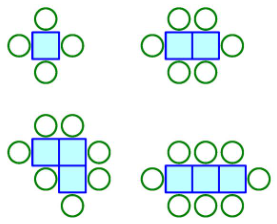
\includegraphics[scale=1]{gametheory10}
            \end{center}
            
            Oleh karena itu, selama $n \le 3$, maka tidak mungkin bagi Rayyan untuk mewarnai setiap kotak bebas, dikarenakan Rayyan telah mewarnai tepat $2n$ kotak menjadi merah. Dapat disimpulkan bahwa algoritma ini bisa berhenti saat $n \ge 4$.

            \item \textbf{Algoritma Rayyan untuk mencegah Budi mendapatkan lebih dari 4 kotak satuan}\\
            Partisi grid tersebut menjadi bagian-bagian berisi persegi-persegi berukuran $2 \times 2$, yang selanjutnya akan kita sebut sebagai "jendela". Setiap kali Budi mewarnai kotak $c$, maka Rayyan dapat mewarnai kotak yang bertetangga (tepat bersebelahan) di dalam jendela tersebut, lalu mewarnai kotak yang tersisa menjadi merah. Perhatikan bahwa dari konstruksi tersebut,  jelas bahwa pada setiap jendela, tidak ada dua kotak biru yang saling bertetangga.

            Akan ditunjukkan bahwa konstruksi tersebut membatasi setiap poligon untuk memiliki maksimal 4 kotak biru. Misalkan beri label sebuah kotak biru $w$, dan WLOG asumsikan kotak $w$ berada tepat di sebelah kanan bawah suatu jendela. Beri label kotak $x,y,z$ pada sebelah kanan, bawah, dan kanan bawah dari kotak $w$ seperti gambar berikut.

            \begin{center}
                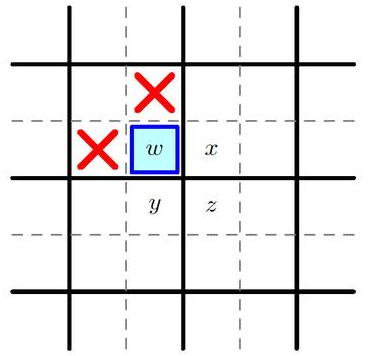
\includegraphics[scale=1]{gametheory10(1)}
            \end{center}
            
            Dari konstruksi tersebut, mudah disimpulkan bahwa poligon biru tidak bisa lebih luas daripada daerah yang ditempati oleh $\{w,x,y,z\}$, dikarenakan jika salah satu kotak tersebut berwarna biru, maka kotak yang bertetangga pasti berwarna merah. Dari sini didapatkan bahwa Rayyan dapat membuat poligon yang dibuat Budi paling besar memiliki luas 4.
        \end{itemize}
        Dari kedua fakta tersebut, didapatkan bahwa skor terbesar yang mungkin didapat Budi adalah 4.
    \end{solusi}
\end{soaljawab}

% \begin{soaljawab}
% % The Niels Henrik Abel 2023
%     Aqua dan Ruby sedang bermain sebuah permainan dengan awalnya diberikan bilangan bulat $m$ dan $n$ dengan $n \ge 4$ dan $m \le 2n+1$. Aqua mulai dengan memilih sebuah bilangan dari himpunan $\{1,2,\dots,n\}$, lalu menulisnya di papan tulis. Selanjutnya, Ruby memilih bilangan lain dari himpunan yang sama dan menulisnya di papan tulis. Mereka melakukan hal itu secara bergiliran dengan memilih bilangan yang belum pernah ditulis di papan tulis. Saat jumlah semua bilangan di papan tulis bernilai lebih dari sama dengan $m$, permainan berakhir, dan siapapun yang menulis bilangan terakhir dinyatakan sebagai pemenang. Berapa banyak kombinasi $m$ dan $n$ sehingga Aqua mempunyai strategi menang?
%     \begin{solusi}
        
%     \end{solusi}
% \end{soaljawab}

\end{document}
